\chapter{Pruebas}
En este capitulo se muestran los resultados de las pruebas realizadas sobre el prototipo 10. Las pruebas realizadas fueron de tiempo de respuesta y de trafico de información en la red.
\section{Prueba de rendimiento, Cifrado y Descifrado de un solo CAPTCHA}
En la figura \ref{fig:7-1} se muestra la relación de metodos que permiten el cifrado del mensaje y la generación de un solo CAPTCHA. El tiempo total que tarda en hacer todo el proceso es de 0.17s donde las funciones que tardan mas en realizar sus tareas son Ek\_din.crearCAPTCHA que se encarga de crear el CAPTCHA y la función Ek\_din.primoSig que calcula el numero primo mas cercano dependiendo del tamaño del CAPTCHA a realizar.\\\\
En la figura \ref{fig:7-2} se muestra la relación de metodos que permiten el descifrado del mensaje, este proceso es muy sencillo para un solo CAPTCHA ya que lo que introduce en usuario es lo que se canvierte en la clave de descifrado. El tiempo que tarda este proceso es de 0.004s.
\begin{figure}[H]
 \centering
 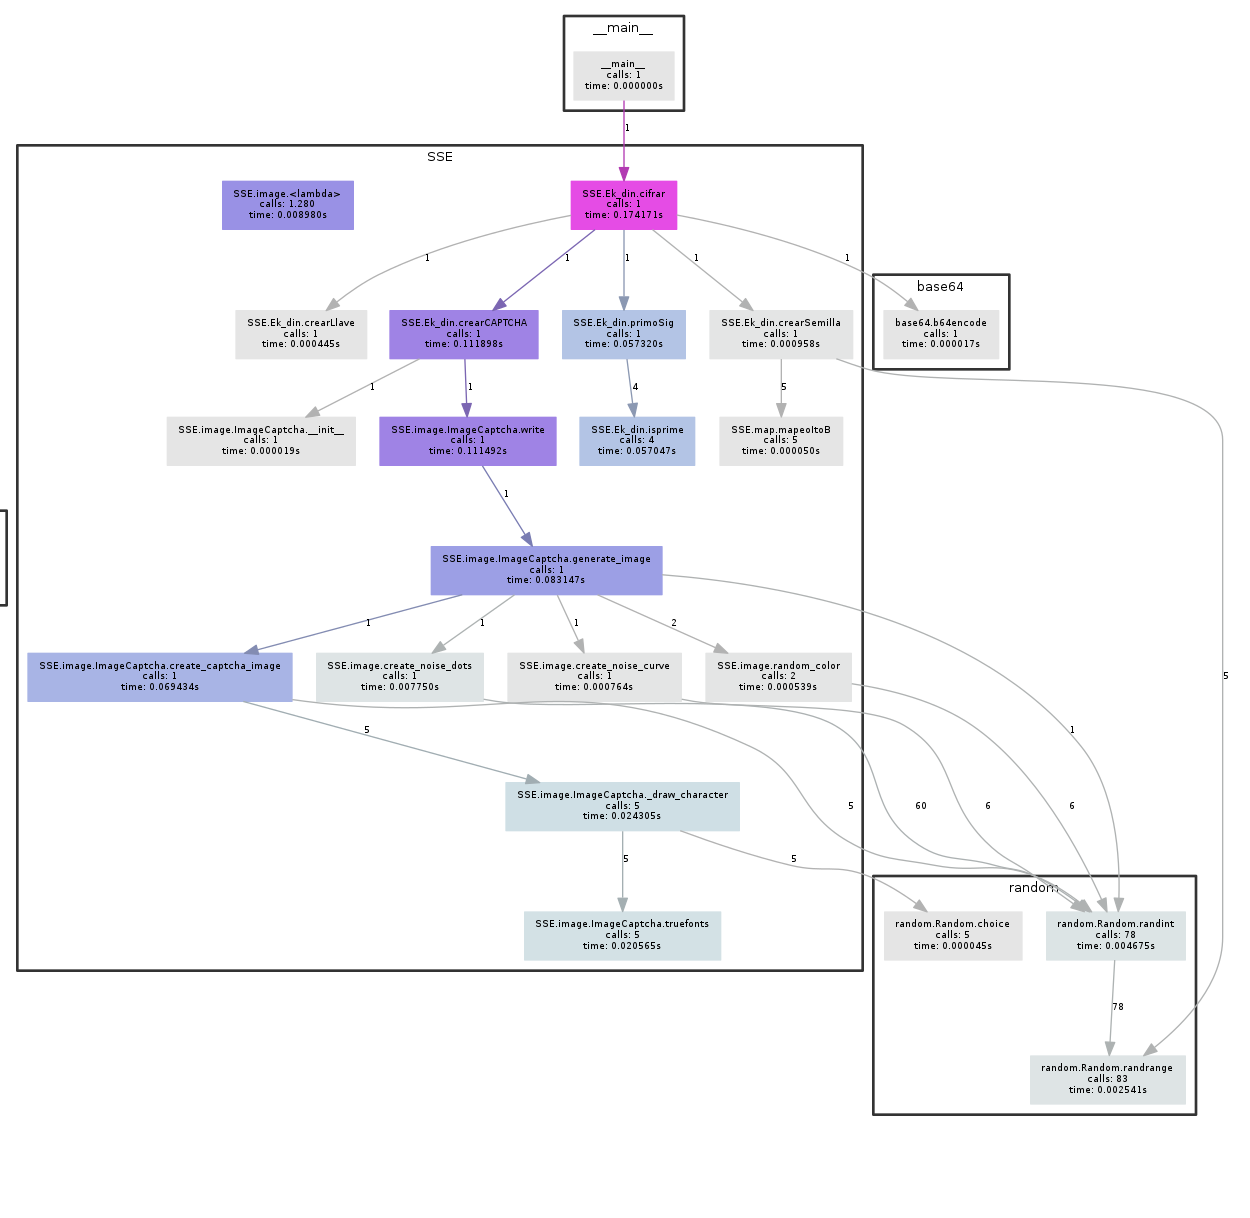
\includegraphics[height=7in]{./images/idda_unic.png}
		\caption{Rendimiento del esquema para un solo CAPTCHA}
		\label{fig:7-1}
\end{figure}

\begin{figure}[H]
 \centering
 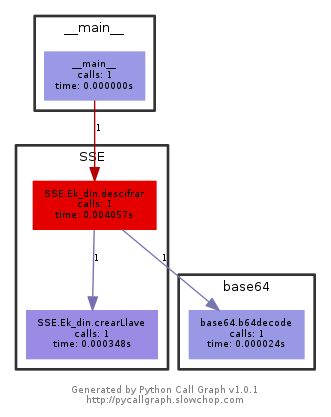
\includegraphics[height=6.3in]{./images/regreso_uni.png}
		\caption{Rendimiento del esquema para un solo CAPTCHA}
		\label{fig:7-2}
\end{figure}
\section{Prueba de rendimiento, Cifrado y Descifrado de multiples CAPTCHA's}
En la figura \ref{fig:7-3} se encuentra la relación de funciones que generan múltiples CAPTCHAS y cifran el mensaje, en este caso la llamada a funciones es mayor que para un solo CAPTCHA, se puede ver que al igual que en el esquema de un solo CAPTCHA las funciones que mas tardan son las de Ek\_din.crearCAPTCHA  y la función Ek\_din.primoSig dandonos un tiempo total para todo el proceso de 0.47s.\\\\
En la figura \ref{fig:7-4} se encuentra la relación de funciones que resuelve el algoritmo de secreto compartido y descifra el mensaje, este es mas elaborado que el descifrado para un solo CAPTCHA en este la función que mas tarda es Ek\_din.primoSig por el tamaño de numero que esta manejando, el tiempo total de termino de la tarea es 0.062s.
\begin{figure}[H]
 \raggedright
 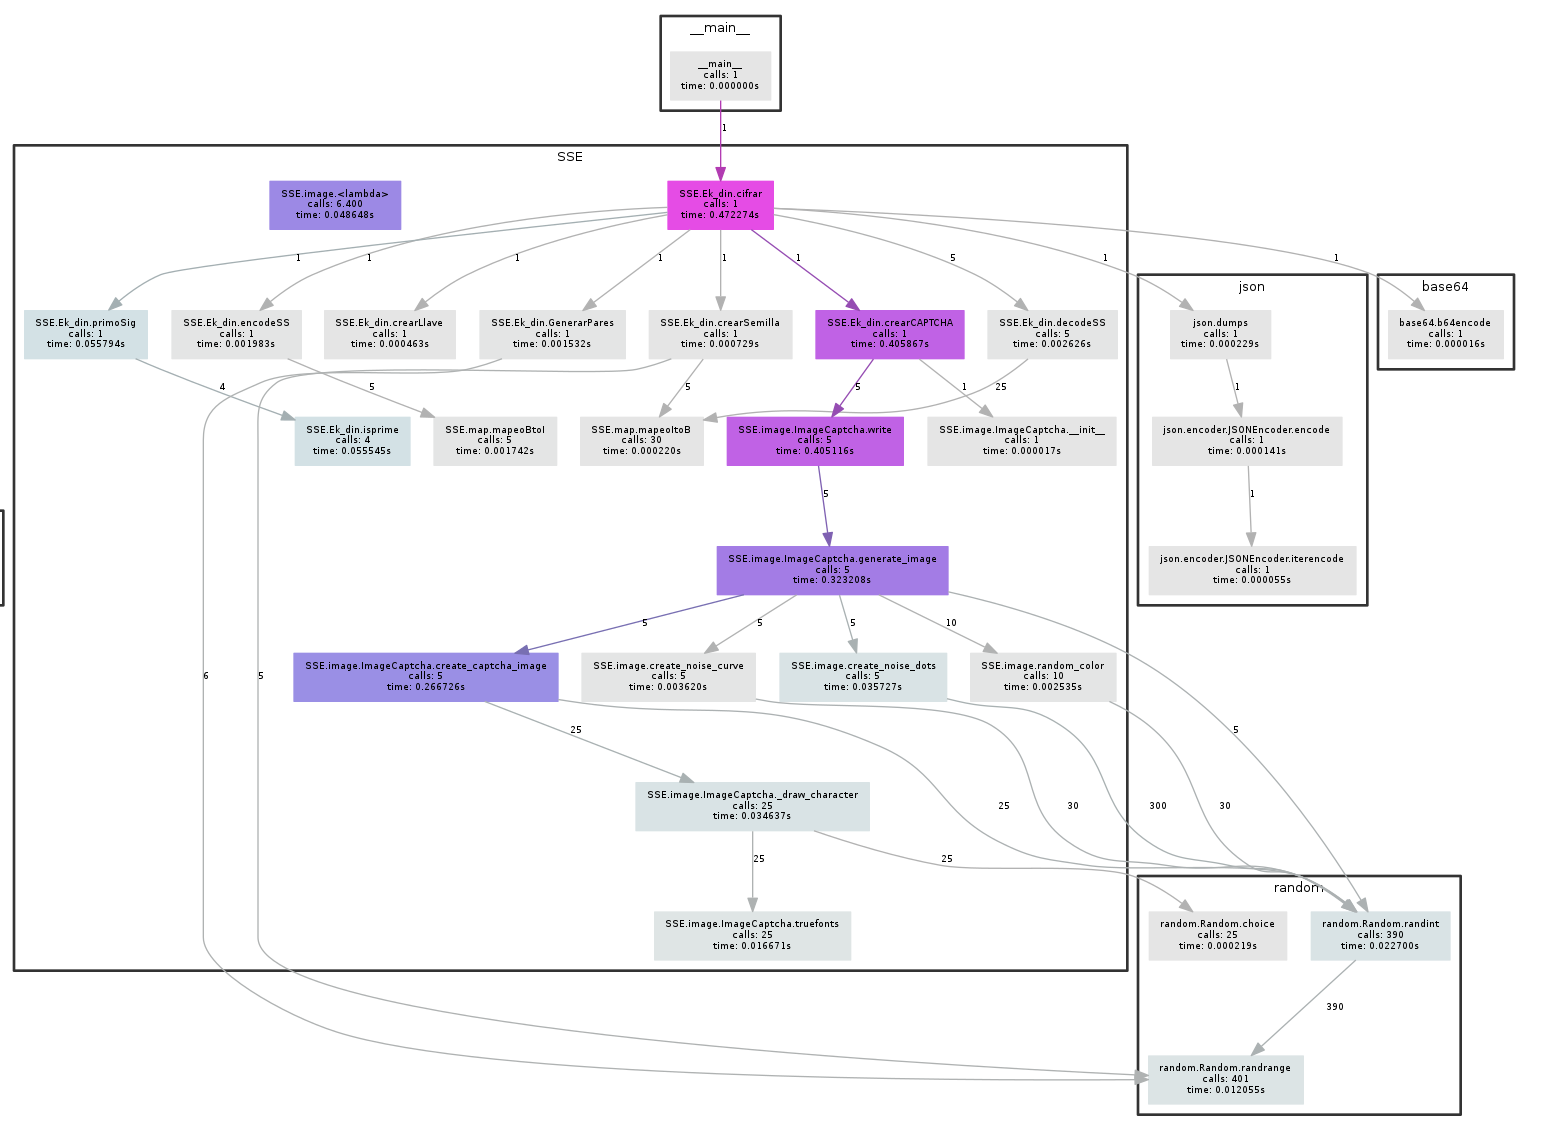
\includegraphics[height=5.5in]{./images/idda_multic.png}
		\caption{Rendimiento del esquema multiCAPTCHA}
		\label{fig:7-3}
\end{figure}
\begin{figure}[H]
 \raggedright
 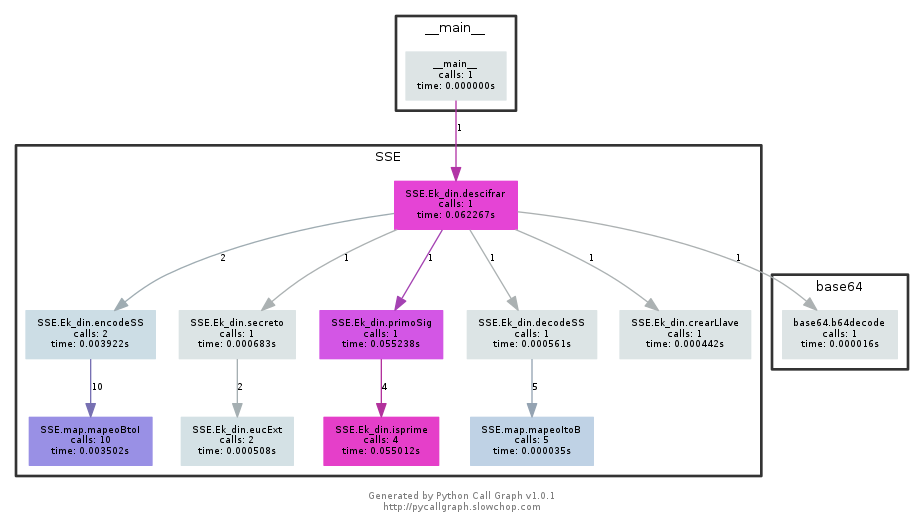
\includegraphics[height=4in]{./images/regraso_multi.png}
		\caption{Rendimiento del esquema multiCAPTCHA}
		\label{fig:7-4}
\end{figure}